\chapter{Diseño}
\label{design}

\section{Referencias}
En esta sección se encuentran aquellas aplicaciones que, tras una revisión de los mismos, se cree que han sido de utilidad por su parecido a la hora de desarrollar este proyecto:

\subsubsection{My OldBoy!}

\textbf{My OldBoy!} es un emulador de Game Boy y Game Boy Color diseñado específicamente para dispositivos Android, que destaca por su precisión en la emulación de casi todos los aspectos del hardware original. Además de simular las consolas, soporta características especiales como el uso del cable link, la vibración y el sensor de inclinación.
\\\\
El emulador es altamente valorado por su interfaz intuitiva y las múltiples opciones de personalización, que incluyen la posibilidad de añadir colores a juegos monocromáticos y modificar la disposición y el tamaño de los controles en pantalla. Entre las ventajas que ofrece, están la alta compatibilidad con juegos y la capacidad de ajustar la velocidad del juego, tanto para avanzar rápidamente como para ralentizarlo en momentos difíciles.
\\\\
Sin embargo, tiene algunas limitaciones. Por ejemplo, puede generar archivos de guardado duplicados, carece de un sistema de autoguardado periódico y no ha recibido actualizaciones recientes para las versiones más nuevas de Android, lo que puede afectar su compatibilidad en dispositivos más modernos.

\begin{figure}[H]
    \centering
    
\includegraphics[width=0.3\textwidth]{include/images/myoldboy.png}
    \caption{My OldBoy! - Logotipo.}
    \label{figure:oldboylogo}
\end{figure}

La pantalla principal de la aplicación presenta un explorador de archivos que muestra, en formato de lista, los documentos almacenados en la carpeta especificada de la memoria interna del dispositivo. Los archivos se organizan automáticamente por orden alfabético, ofreciendo una visualización clara y estructurada para facilitar su navegación y selección. Dispone de dos botones, uno para recargar la carpeta actual y otro para acceder a los ajustes de sistema. 
\\\\
En los ajustes, podremos modificar distintos aspectos agrupados en las categorías de video, audio, datos de entrada, disposición, varios y avanzado. En vídeo, por ejemplo, podremos modificar el tamaño de la pantalla de juego, la orientación predeterminada de la aplicación, o la paleta de colores.

\begin{figure}[H]
    \centering
    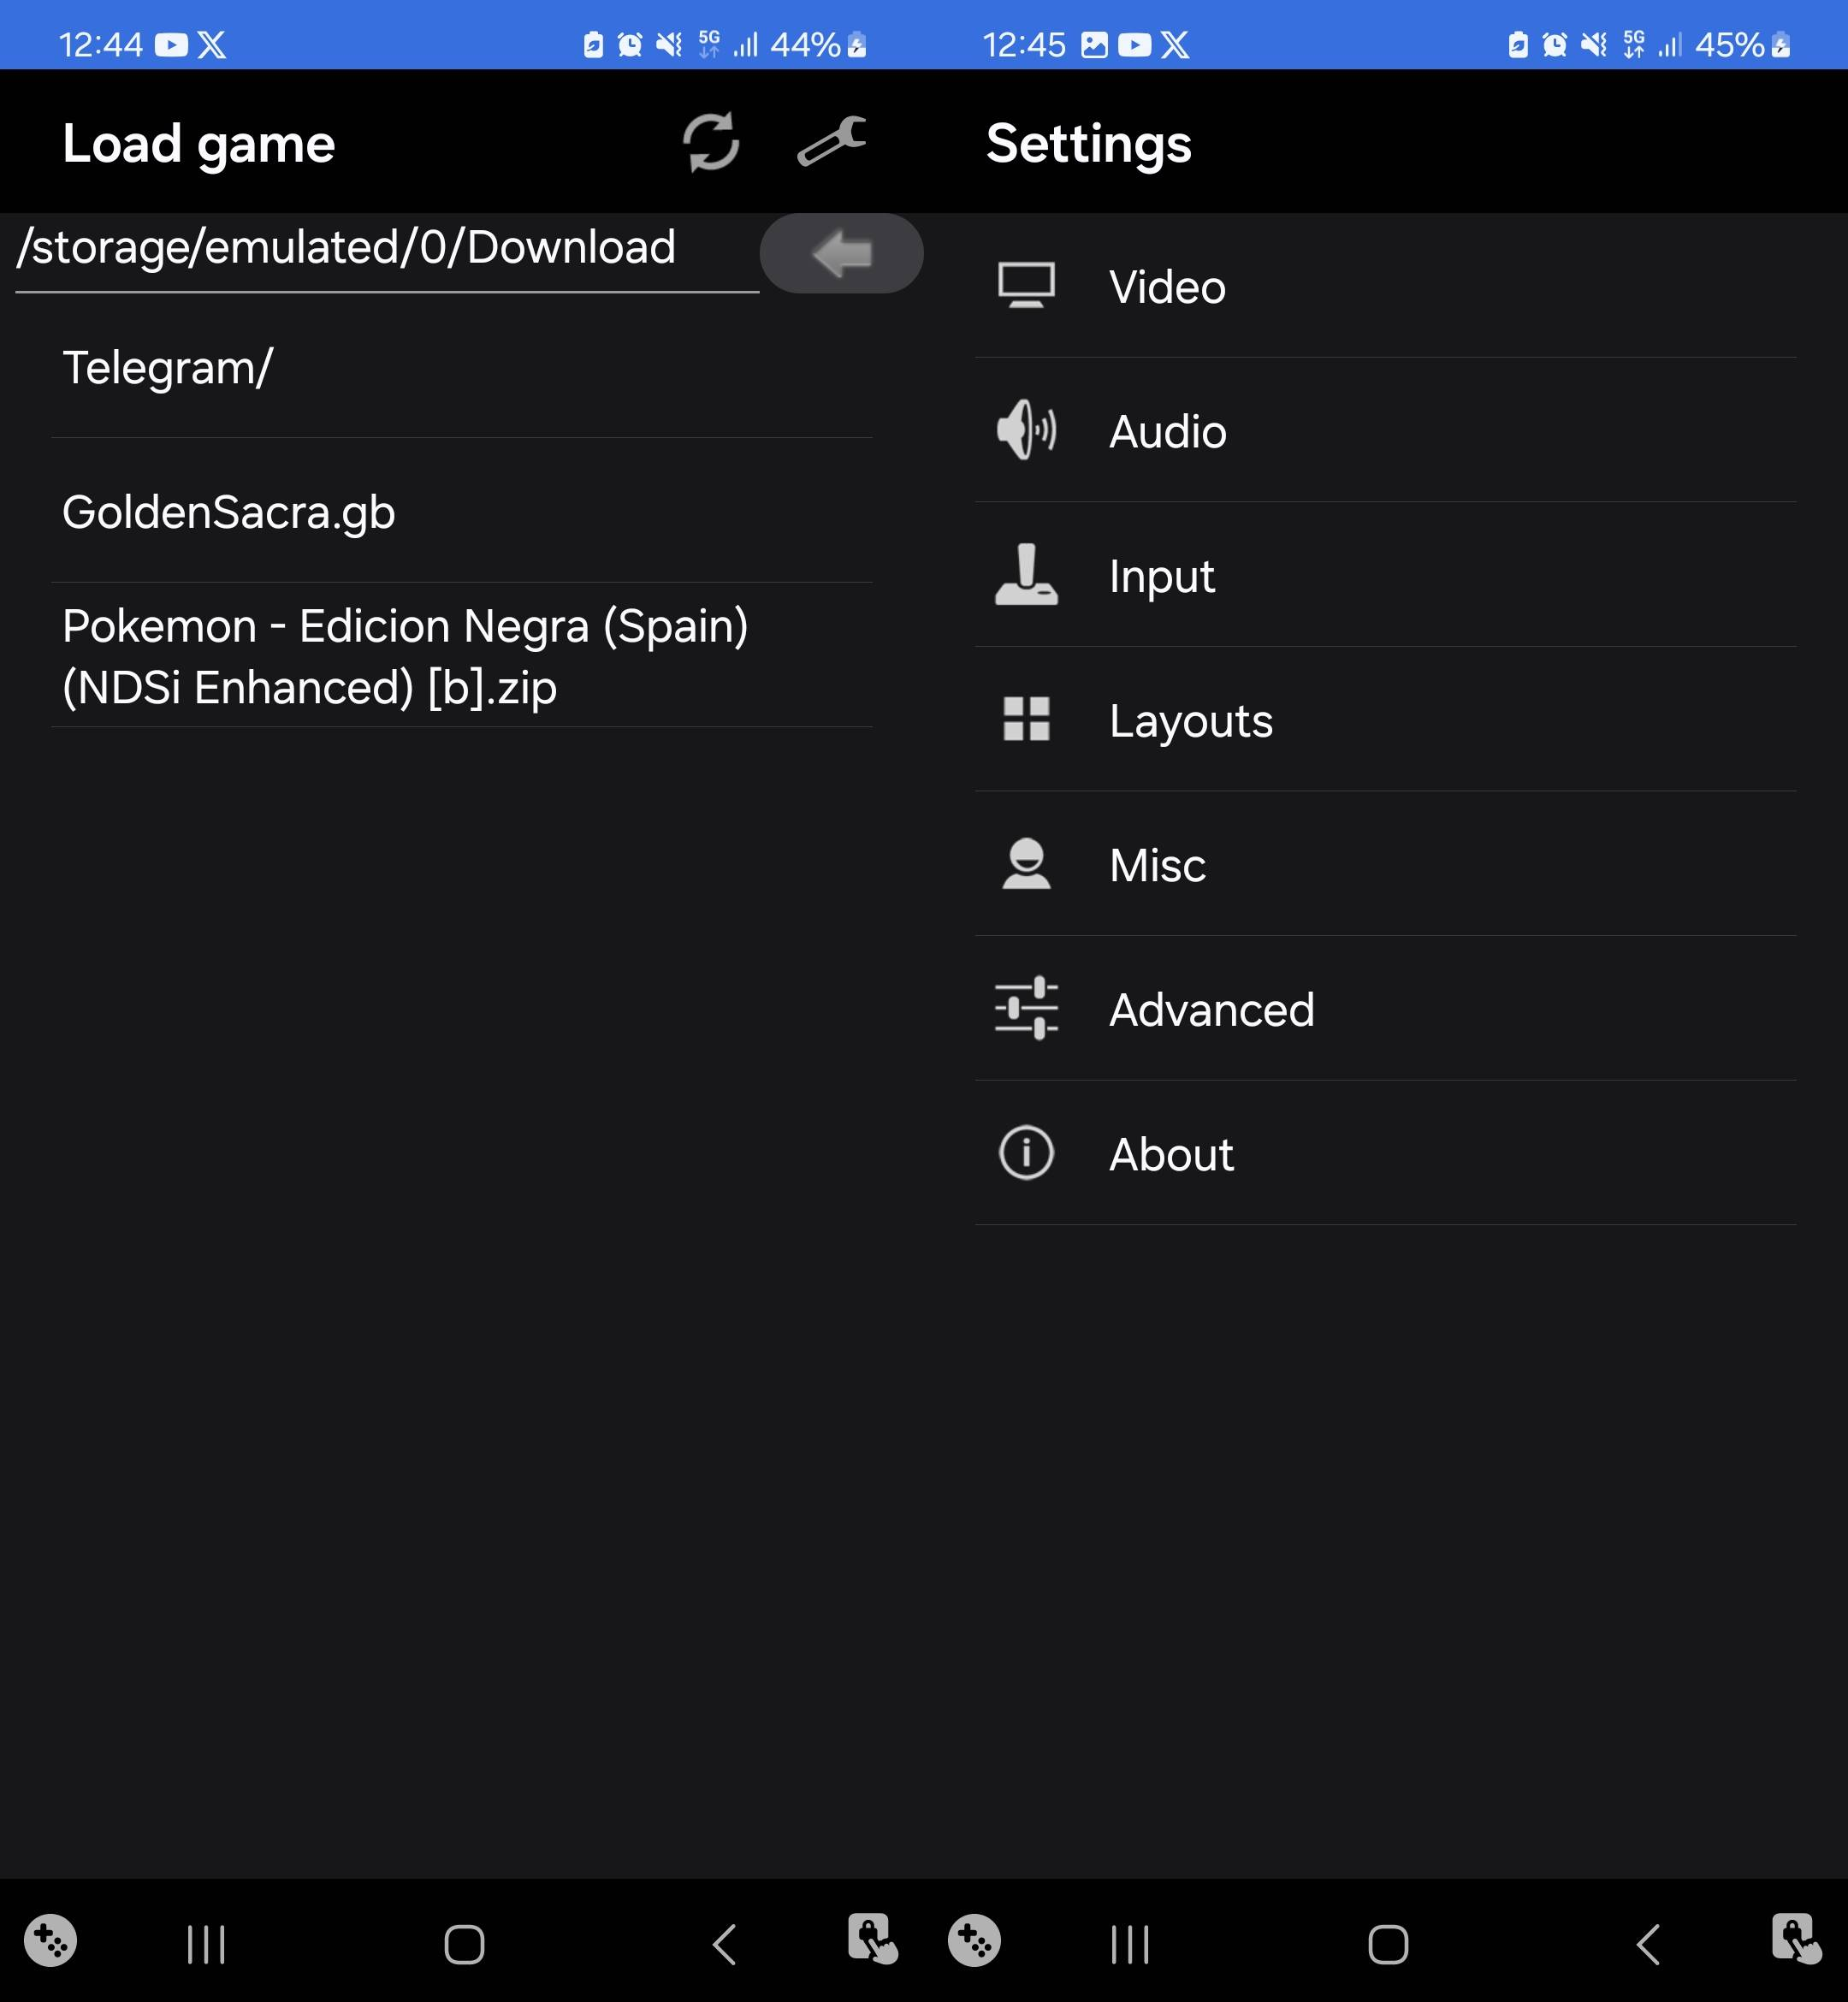
\includegraphics[width=0.6\textwidth]{include/images/myoldboy2.jpg}
    \caption{My OldBoy! - Menú de inicio y pantalla de ajustes.}
    \label{figure:oldboy2}
\end{figure}

\begin{figure}[H]
    \centering
    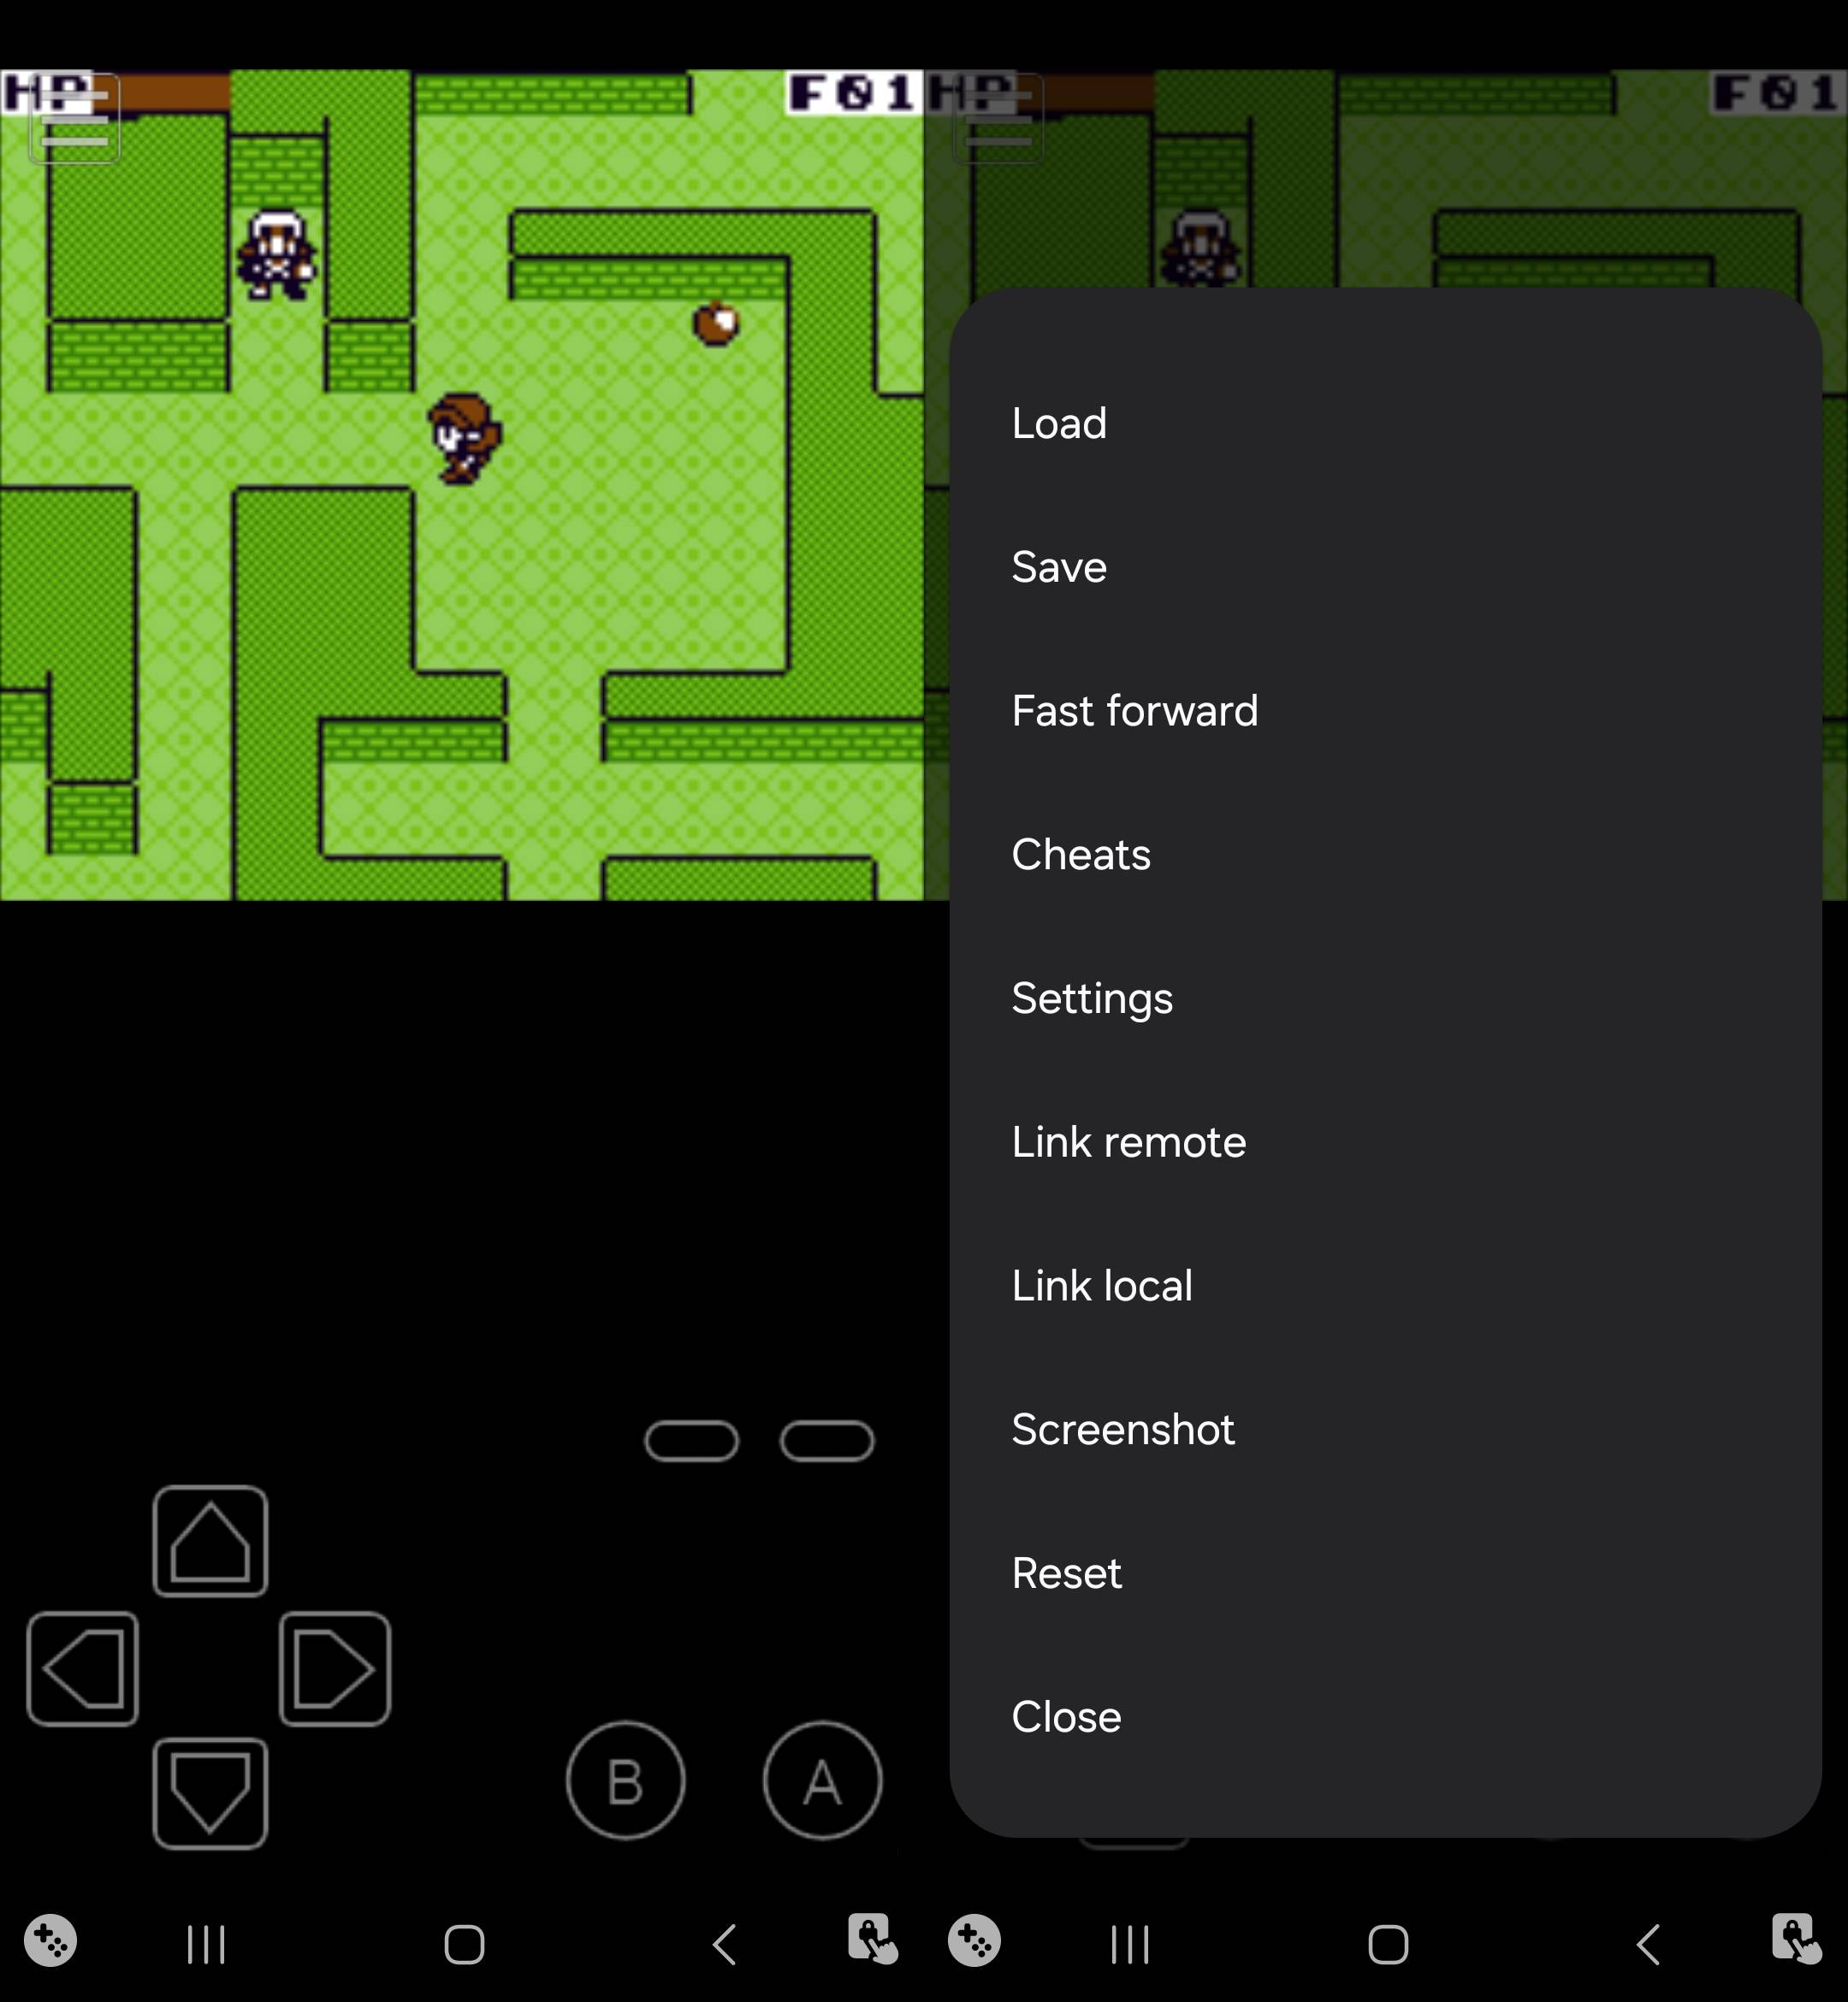
\includegraphics[width=0.6\textwidth]{include/images/myoldboy3.jpg}
    \caption{My OldBoy! - Pantalla y opciones de juego.}
    \label{figure:oldboy3}
\end{figure}


\subsubsection{GBCC}

\begin{figure}[H]
    \centering
    
\includegraphics[width=0.6\textwidth]{include/images/gbcclogo.png}
    \caption{GBCC - Logotipo.}
    \label{figure:gbcclogo}
\end{figure}

\subsubsection{iGBA}

\begin{figure}[H]
    \centering
    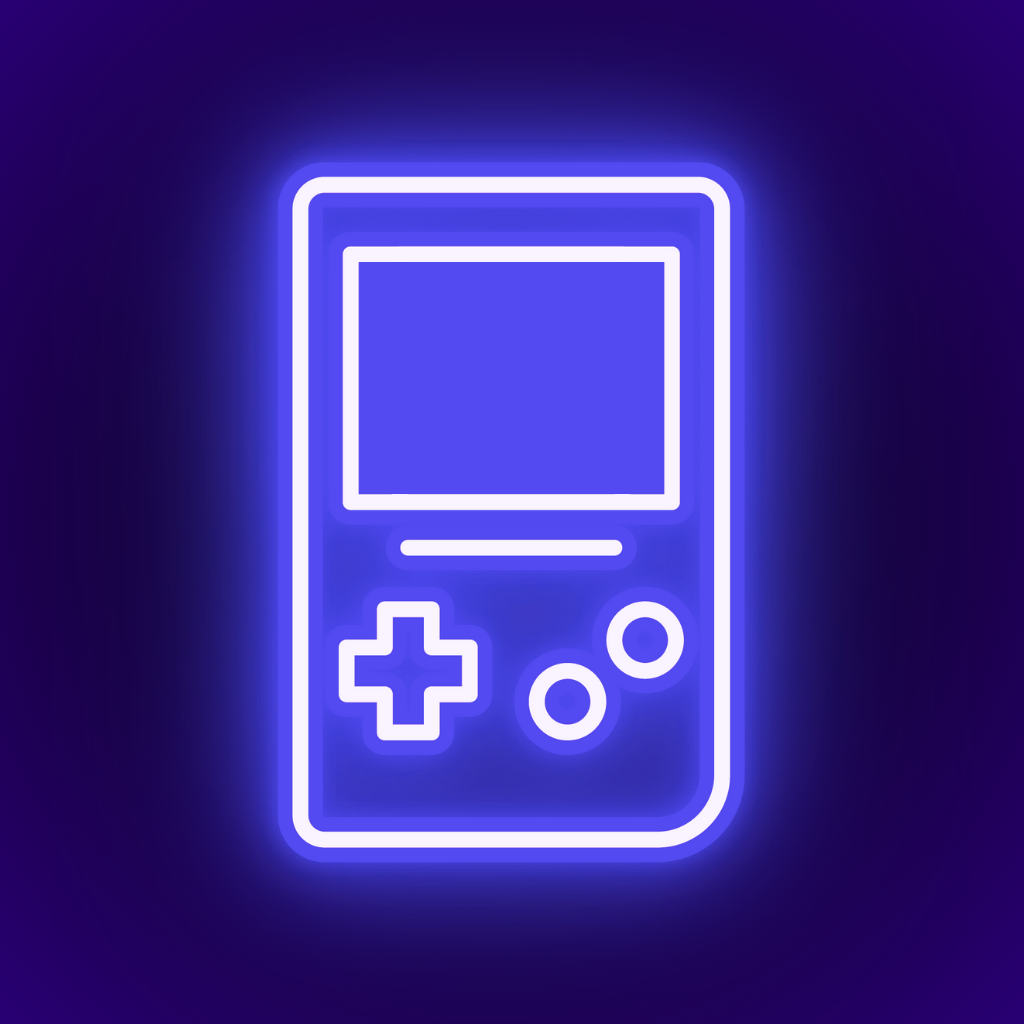
\includegraphics[width=0.4\textwidth]{include/images/igbalogo.png}
    \caption{iGBA - Logotipo.}
    \label{figure:igbalogo}
\end{figure}

\section{Mockup}

\begin{figure}[H]
    \centering
    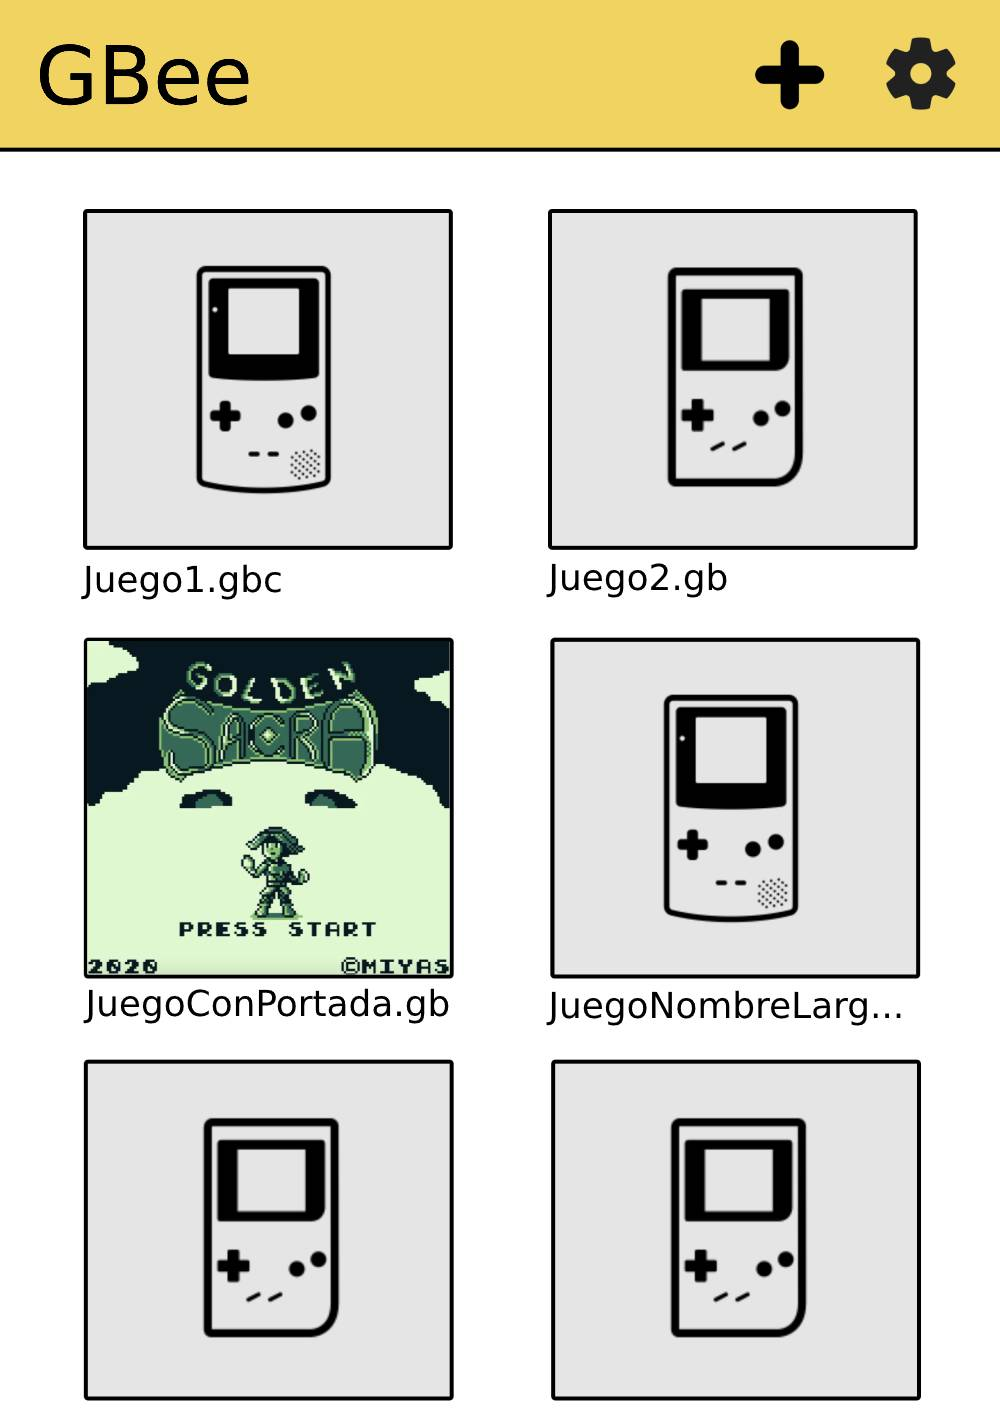
\includegraphics[width=0.4\textwidth]{include/images/mockup_menu.jpg}
    \caption{Menú de inicio.}
    \label{figure:mockupmenu}
\end{figure}

\begin{figure}[H]
    \centering
    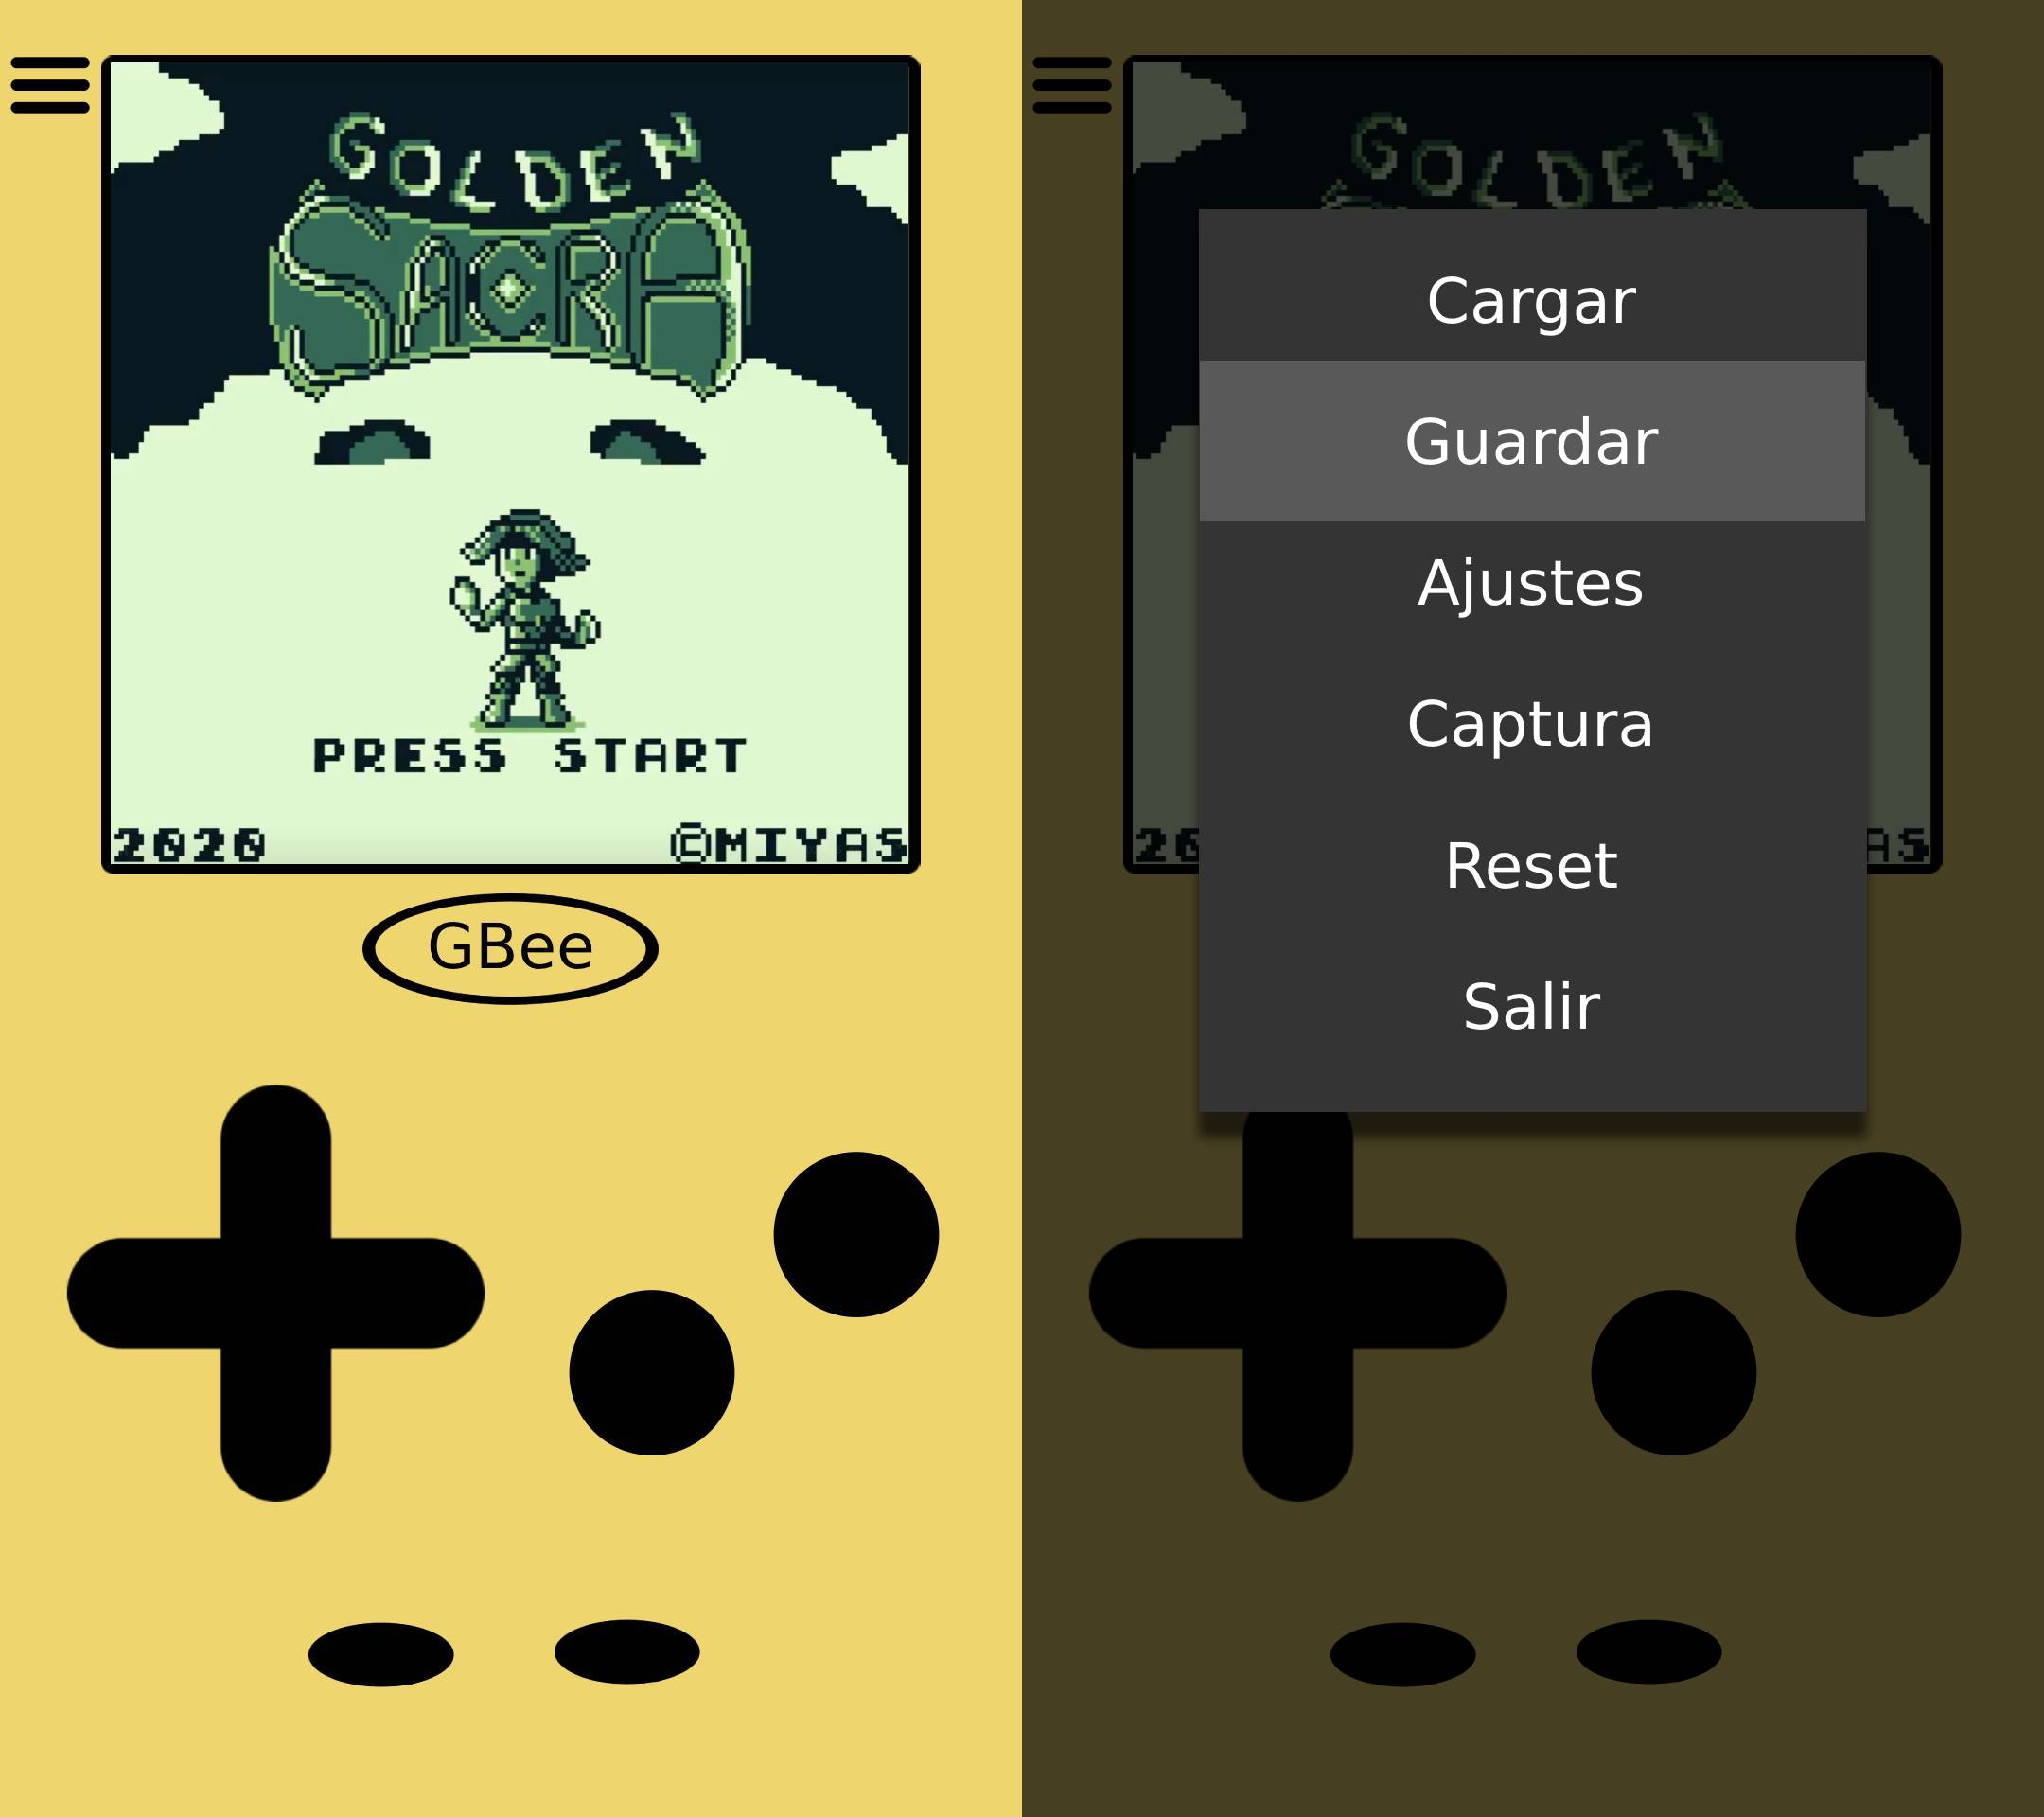
\includegraphics[width=0.6\textwidth]{include/images/mockgame.jpg}
    \caption{Pantalla de juego.}
    \label{figure:mockupgame}
\end{figure}

\section{Diagrama de casos de uso}

\cleardoublepage